%
%                  Politecnico di Milano
%
%         Student: Caravano Andrea, Cantele Alberto
%            A.Y.: 2024/2025
%
%   Last modified: 19/03/2025
%
%     Description: Internet of Things: Challenge n. 1
%                  Implementation report
%

\documentclass[a4paper,11pt]{article} % tipo di documento
\usepackage[T1]{fontenc} % codifica dei font
\usepackage[utf8]{inputenc} % lettere accentate da tastiera
\usepackage[english,italian]{babel} % lingua del documento
\usepackage{lipsum} % genera testo fittizio
\usepackage{url} % per scrivere gli indirizzi Internet e/o di riferimento nella pagina

\usepackage[hidelinks]{hyperref} % per modificare il comportamento dei collegamenti ipertestuali (+ leva colore attorno)

\usepackage[margin=0.7in]{geometry} % margine di pagina

\usepackage{graphicx} % per inserire immagini

\usepackage[outputdir=../auxil]{minted} % per colorazione automatica del codice (installare pygments da Homebrew)
% \usepackage{pythonhighlight} % per Python

\setminted{ % si può impostare il linguaggio specifico con \setminted[JSON] ad esempio
    linenos=true,
    breaklines=true,
    encoding=utf8,
    fontsize=\normalsize,
    frame=lines
}

\usepackage{fancyhdr}
\usepackage{textcomp}
\usepackage{siunitx} % per gestione intestazione e piè di pagina

\hypersetup{ % metadati di titolo e autore nel PDF
    pdftitle={Internet of Things: Challenge n. 1},
    pdfauthor={Andrea Caravano, Alberto Cantele}
}

\setlength{\parindent}{0pt} % rimuove l'indentazione del testo

\begin{document}
    \pagestyle{fancy}
    \fancyhead{}\fancyfoot{}
    \fancyhead[L]{\textbf{Internet of Things: Challenge n. 1}}
    \fancyhead[R]{Andrea Caravano, Alberto Cantele}
    \fancyfoot[C]{\thepage}

    \title{\textbf{Internet of Things}\\Challenge n. 1: Implementation report}
    \author{Andrea Caravano, Alberto Cantele}
    \date{Academic Year 2024--25}
    \maketitle


    \section{Implementation and design choices}\label{sec:implementation-and-design-choices}

    The code is organized into small sub-functions to enhance clarity and generalize the behaviour with respect to the real board, also if not only emulated.

    The overall structure is roughly described as follows.
    Deeper explanation is then expanded for the most relevant elements.

    \begin{itemize}
        \item The \texttt{loop} function is empty because of the employment of the Deep Sleep technique.

        Once the board reboots, in fact, the \hyperref[setup]{\texttt{setup}} function is immediately called.
        Therefore, it is convenient to exploit it directly.

        The specification requires that a single measurement is sent by the node once every deep sleep interval \hyperref[subsubsec:higher-duty-cycle]{(see following calculations)}.
        \item The \texttt{WiFi\_initialization} function receives in input a peerStructure, used to register the peer that the sender node is connected to.

        In the emulation environment, it is represented by the virtual board itself, using the defined broadcast address.

        The Wi-Fi module of the board is turned on and prepared for usage via \textsc{ESP-NOW} (an ESP-32 specific implementation).

        The \textsc{callbacks} functions are then registered for usage via the \textsc{send} or \textsc{receive} event activation, therefore triggered.

        Transmission power is finally set to 2 dBm, which is the minimum value for the parameter possible \hyperref[subsec:transmission-power-regulation]{(see considerations in the energy consumption part)}.
        \item The \texttt{sendMessage} function simply uses \textsc{ESP-NOW} bindings to invoke the send action.

        The message is sent in textual form and converted to a byte array for network transfer, specifying the occupancy state of the parking slot.
        \item The \texttt{OnDataSent} callback function is called upon a send event via \textsc{ESP-NOW} and checks for transmission errors.

        In case transmission is successful, no serial prints are produced, as they are not useful in the emulation environment.
        \item The \texttt{OnDataRecv} callback function is called upon a reception event via \textsc{ESP-NOW} and plays the role of the sink node receiving the occupancy status of the parking slot.

        Result of the distance computation produced by the sender node is print in output via the Serial monitor.
        \label{ultrasonic-distance-measurement}
        \item The \texttt{elaborateMessage} function produces the distance measurement via the \textsc{HC-SR04 Ultrasonic Distance Sensor}.

        As per the documentation examples, the measurement cycle requires to start setting initially the \textsc{TRIGGER} PIN to \textsc{LOW}, then expressing the intention to start a measurement writing an \textsc{HIGH} value for (at least) 10 \mu s.

        The \textsc{TRIGGER} can finally be reset to \textsc{LOW}.

        The distance measurement is proportional to the duration of \textsc{ECHO} PIN pulse, so the conversion factor is taken into account when doing the final evaluation and selection of the occupancy status.

        \label{setup}
        \item The \texttt{setup} function is executed each time the board is woken up from the Deep Sleep state or initialized for the first time.

        As usual, it prepares the Serial Console and the related Baud Rate.

        It specifies the PINs behaviour and links the other function invocations to the overall behaviour of the node, being detecting the parking occupancy status and informing the sink node of it.

        It finally computes the Wakeup timer for the Deep Sleep state and enters it, at the end of the function.

        It will be repeated at the board Wakeup.
    \end{itemize}


    \section{Energy computations and plots}\label{sec:energy-computations-and-plots}

    \subsection{The datasets and the important figures of merit}\label{subsec:the-datasets-and-the-important-figures-of-merit}

    In the Python notebook provided as a complement to the report, the biggest focus of the examination was put on the CSV files provided with the task's specifications, among a newly-crafted one, derived from the board's code instrumentation.

    In fact, a particular constant value in the code enables instrumentation, upon toggling of the truth boolean value:

    \begin{minted}{C++}
#define TIME_MEASUREMENT_INSTRUMENTATION true
    \end{minted}

    The main aspects to consider in the consumption analysis are:
    \begin{itemize}
        \item Power consumption analysis: starting from the provided CSV files, averaging meaningful values among the ones concerning each algorithm's phase.
        \item Time estimation: starting from the detected measurements in the emulation environment, the goal is to determine the average duration of each algorithm's phase, excluding possible outliers, caused by the emulation overhead.
        \item Energy estimation: combination of the previous ones, resulting in the energy consumption by the board over time.
    \end{itemize}

    \subsection{Power consumption analysis}\label{subsec:power-consumption-analysis}

    In the provided dataset, the following figures of merit have been isolated.

    \begin{itemize}
        \item \textsc{Deep Sleep state}: The board enters a specific power-save status in which most components are turned off to minimize power consumption and therefore preserving battery lifetime.

        This is reflected in the following histogram, where theoretical expectations are met, resulting in the lowest possible power consumption state.
        \item \textsc{Idle phase}: The board is not providing useful computation, but its processing unit is still running and some components are still on, wasting some energy.

        The idle phase is composed of two parts:
        \begin{enumerate}
            \item Between the beginning of the execution and the beginning of the Sensor Reading phase.
            \item Between the end the Sensor Reading phase and the Wi-Fi chip beginning its initialization.
        \end{enumerate}
        \item \textsc{Wi-Fi Running phase}: The read value is ready for transmission with \textsc{ESP-NOW}.

        The Wi-Fi chip and (emulated) peer structure is populated, the message is transmitted and the chip turned off.

        The chosen transmission power here is 2 dBm \hyperref[subsec:transmission-power-regulation]{(see also the possible improvements section comment on the choice of a reasonable value)}.
        \item \textsc{Transmission phase}: included in the Wi-Fi Running phase itself, being of course part of it, where the pre-computed message is transmitted using the defined transmission power.
        \item \textsc{Sensor Reading phase}: The HC-SR04 Ultrasonic Distance Sensor is activated and the pulse measurement is started \hyperref[ultrasonic-distance-measurement]{(see earlier definition)}, resulting in the distance from the sensor, used to determine the final occupancy state of the parking slot.
    \end{itemize}
    Note that the transmission and Wi-Fi running phase are divided because of the different energy consumption: a peak in the consumed power is present in the Transmission phase.

    As it will be clearly demonstrated via the following calculations, a huge importance is played by the time spent in each phase, rather than its peak value.

    Average resulting values are summarized in the table below.

    \smallskip

    \begin{center}
        \begin{tabular}{|c|c|}
            \hline
            \multicolumn{2}{|c|}{Power consumption analysis} \\
            \hline
            Deep Sleep state           & 59,62 mW  \\
            \hline
            Idle phase                 & 310,97 mW \\
            \hline
            Wi-Fi running phase        & 704,22 mW \\
            \hline
            Transmission phase (2 dBm) & 797,29 mW \\
            \hline
            Sensor reading phase       & 466,74 mW \\
            \hline
        \end{tabular}
    \end{center}

    \smallskip

    Overall, in the resulting histogram, theoretical expectations are completely met.

    \medskip

    \begin{center}
        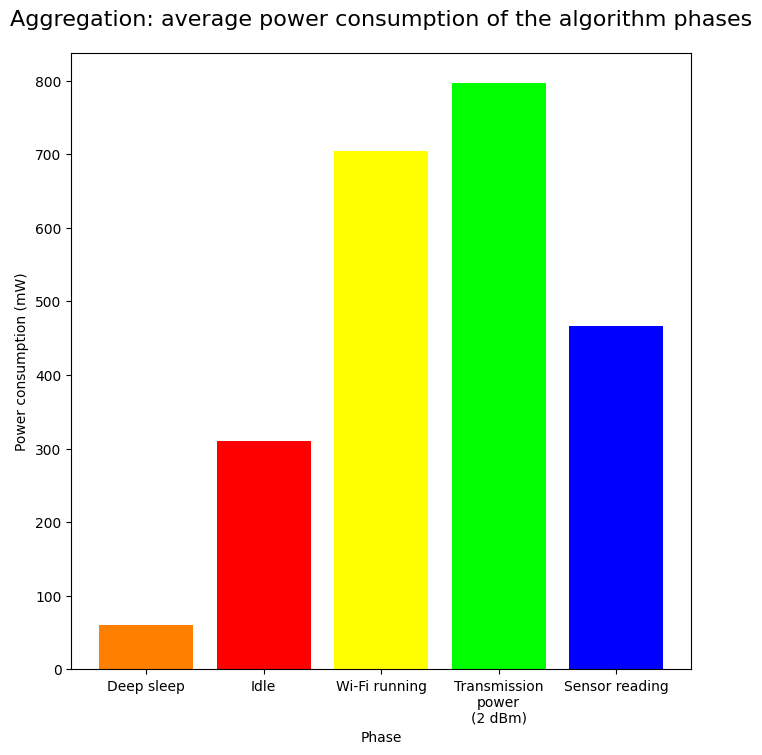
\includegraphics[width=10cm]{../res/power_consumption}
    \end{center}

    \subsection{Time estimation}\label{subsec:time-estimation}
    The most important part of the whole consumption detection job is the subdivision of the algorithm phases, isolating each sub-computation or state, also considering the \hyperref[sec:implementation-and-design-choices]{sketched functional structure defined earlier}.

    Data is in fact aggregated according to differences computed between each phase: each one is made up of the mean of all the corresponding steps in all significative executions.

    Finally, outliers caused by the emulation overhead are isolated.

    Average resulting values are summarized in the table below.

    \smallskip

    \begin{center}
        \begin{tabular}{|c|c|}
            \hline
            \multicolumn{2}{|c|}{Power consumption analysis} \\
            \hline
            Deep Sleep state (fixed) & 15 seconds \\
            \hline
            Idle phase               & 2,44 ms    \\
            \hline
            Wi-Fi running phase      & 219,64 ms  \\
            \hline
            Transmission phase       & 0,30 ms    \\
            \hline
            Sensor reading phase     & 24,10 ms   \\
            \hline
            Total active time        & 246,18 ms  \\
            \hline
        \end{tabular}
    \end{center}

    \smallskip

    Overall, in the resulting histogram, theoretical expectations are completely met.

    \medskip

    \begin{center}
        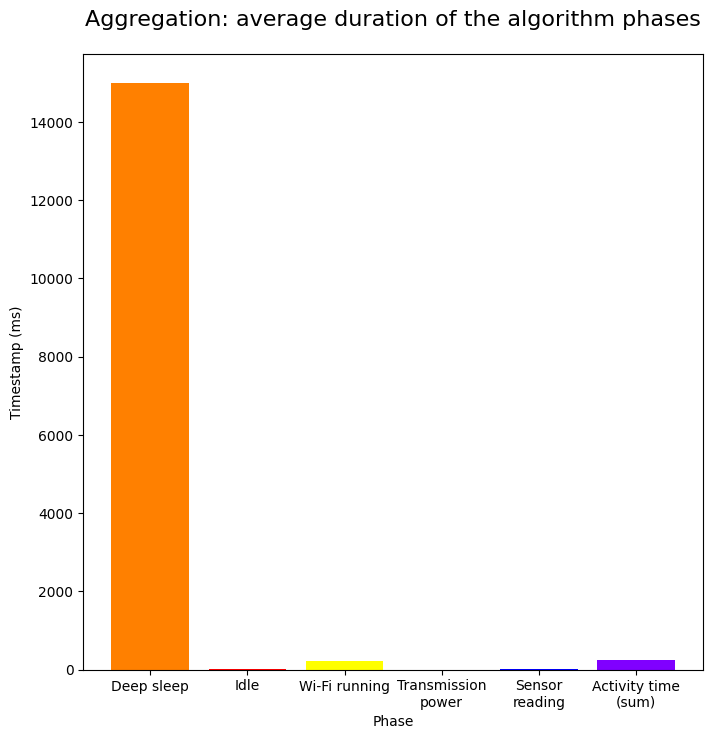
\includegraphics[width=10cm]{../res/time_estimation}
    \end{center}

    By looking at the histogram above, we may start to realize that, even if the Deep Sleep state is the least consuming state energy-wise, we still spend most of our measurement time in it, meaning the difference between the active and the sleeping state may actually turn out to be comparable, in an energy consumption setting.

    Let's discuss it, by completing the estimation.

    \subsection{Energy consumption estimation}\label{subsec:energy-consumption-estimation}

    As a combination of the previous aggregations, the energy consumption is derived from the product of the time spent in each phase and its corresponding average power consumption.

    Average resulting values are summarized in the table below.

    \smallskip

    \begin{center}
        \begin{tabular}{|c|c|}
            \hline
            \multicolumn{2}{|c|}{Energy consumption analysis} \\
            \hline
            Deep Sleep state     & 894,30 mJ \\
            \hline
            Idle phase           & 0,76 mJ   \\
            \hline
            Wi-Fi running phase  & 154,67 mJ \\
            \hline
            Transmission phase   & 0,24 mJ   \\
            \hline
            Sensor reading phase & 11,25 mJ  \\
            \hline
            Total activity       & 166,92 mJ \\
            \hline
        \end{tabular}
    \end{center}

    \smallskip

    The matching histogram is the following, confirming our previous suspects.

    \medskip

    \begin{center}
        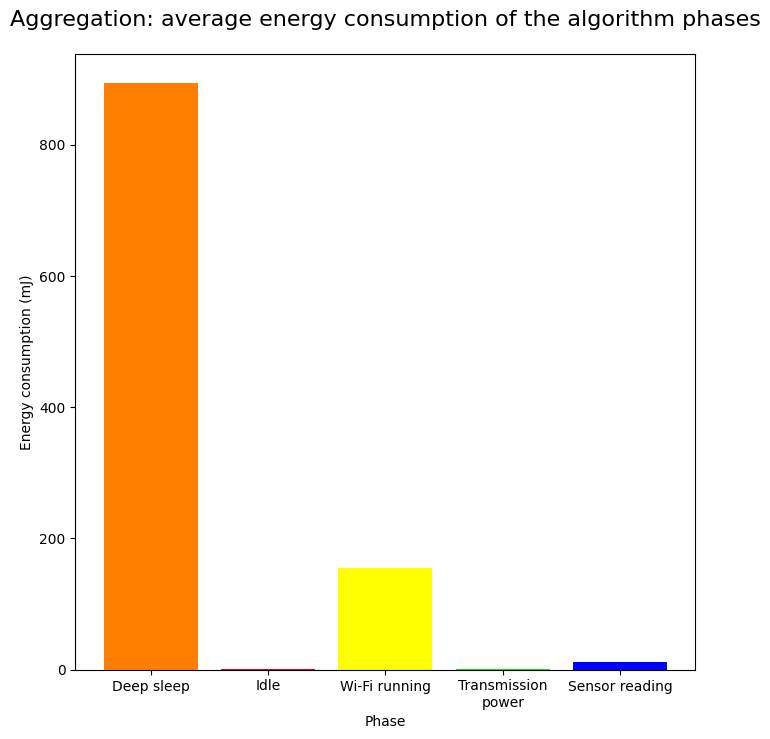
\includegraphics[width=10cm]{../res/energy_consumption}
    \end{center}

    The Deep Sleep state, in fact, is the most prominent one energy-wise.

    This should not come as a surprise, especially considering that it is the most time-consuming state, contributing with a huge difference with respect to overall time durations, even if less power-hungry, overall.

    Let's now compute the resulting lifetime of the board.

    \begin{center}
        \begin{tabular}{|c|c|}
            \hline
            \multicolumn{2}{|c|}{Lifetime computation} \\
            \hline
            Energy budget               & $8260 \% 5000 + 15000$ Joule $= 18260$ Joule \\
            \hline
            Resulting lifetime (cycles) & 17206 cycles                                 \\
            \hline
            Possible activity time      & 258090 seconds \simeq 2 days                 \\
            \hline
        \end{tabular}
    \end{center}

    Possible optimizations would, for sure, begin in the direction of reducing the usage of the Wi-Fi chip and are considered in the last part of the document.


    \section{Improvements proposals and possible revisions}\label{sec:improvements-proposals-and-possible-revisions}

    \subsection{The most sensible approach: A versioning system}\label{subsec:the-most-sensible-approach:-a-versioning-system}
    As expected from the theory classes, the most energy-consuming element is confirmed to reside in the Wi-Fi usage (therefore, in the need of transmitting a sample per measurement).

    If, instead, we exploit a non-volatile storage area to store past readings and compare them with a newly performed one, we would be able to send a new message only when a real difference was detected.

    Natural evolutions would take into consideration the implementation field of the board: a few examples are shown in the following.

    \subsubsection{A higher duty cycle}\label{subsubsec:higher-duty-cycle}

    The actual duty cycle, \hyperref[subsec:time-estimation]{as shown}, can be roughly approximated as \simeq 15 seconds.

    As we are dealing with cars movements in a parking slot, changes in the occupancy state are definitely expected to be much less frequent than the duty cycle used in the current implementation.

    Moreover, in the versioning system case, the duty cycle could be dynamically adapted to a recent change, behaving similarly to a sliding window update.

    Lastly, an additional consideration about the usage of the occupancy states should be taken into consideration.

    In a first approximation, a meaningful fixed value could be from 60 to 180 seconds, that are taken as a reference in the following.

    Revising the attached Python notebook, we obtain the following lifetime figures.

    \begin{center}
        \begin{tabular}{|c|c|}
            \hline
            \multicolumn{2}{|c|}{60-seconds duty cycle} \\
            \hline
            Resulting lifetime (cycles) & 4876 cycles                  \\
            \hline
            Possible activity time      & 292560 seconds \simeq 3 days \\
            \hline
        \end{tabular}
    \end{center}

    Less possible cycles are completely expected, as they will last more.
    In fact, a higher activity time is a good sign of a meaningful optimization being achieved.

    Overall, in the resulting histogram, theoretical expectations are completely met.

    \medskip

    \begin{center}
        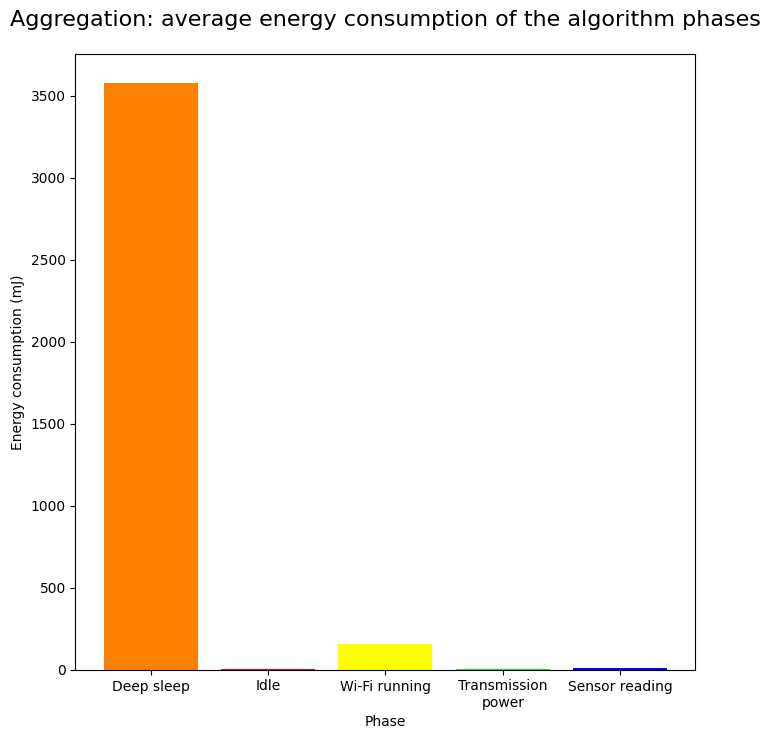
\includegraphics[width=10cm]{../res/60_energy_consumption}
    \end{center}

    \begin{center}
        \begin{tabular}{|c|c|}
            \hline
            \multicolumn{2}{|c|}{180-seconds duty cycle} \\
            \hline
            Resulting lifetime (cycles) & 1675 cycles                  \\
            \hline
            Possible activity time      & 301500 seconds \simeq 3 days \\
            \hline
        \end{tabular}
    \end{center}

    Here, we start to realize that a reasonable threshold has been reached by approaching to a 60 seconds duty cycle.

    Therefore, we should stick to a value near to it (or adapt the measurement cycle correspondingly).

    \subsubsection{Parking activity times}

    As in most parking slots, regular activity times are generally observed, meaning a parking slot is expected to open at a certain morning time and close in the evening.

    In the remaining time, no updates to the status of the slot are expected.

    A specifically crafted night-cycle could in fact be implemented, expanding the duty cycle to a decidedly higher value (\sim 30 minutes, for example).

    Also, remember that the node should keep its internal clock updated (for example, with the NTP protocol via the classical internet) and implement a mechanism to account for extraordinary opening and closure times.

    \subsubsection{Non-volatile storage}

    As shown during the laboratory lectures, a non-volatile variable can be retained among reboots.
    This mechanism can be exploited, for example, to store the latest distance measurement and the duty cycle currently in use.

    \begin{minted}{C++}
RTC_DATA_ATTR float latest; // ex: 75.0 cm
RTC_DATA_ATTR int next_sleep_timer; // ex: 180 seconds
    \end{minted}

    \subsubsection{Keep-alive message}

    The protocol could finally include a new message serving as a heart-beat, for sensors that have not updated their status for at least a pre-defined amount of time, to distinguish
    low-usage periods of the slot from a battery drain, that would require maintenance.

    An example is shown below.
    Note that, of course, an additional factor related to the activity time of the board should be considered.

    In a first approximation attempt, it is accounted with a bonus cycle.

    \begin{minted}{C++}
#define KEEPALIVE_FREQUENCY 30 * 60 // 30 minutes, expressed in seconds
...
RTC_DATA_ATTR int next_sleep_timer = 180; // seconds
RTC_DATA_ATTR int total_sleep_time; // seconds
...
String elaborateMessage() {
        ...
        if (/* no change in the occupancy status ... */ && (total_sleep_time + next_sleep_timer) > KEEPALIVE_FREQUENCY) {
            return "KEEPALIVE"; // The new message of the small application-layer textual protocol
        }
        ...
}
...
void setup() {
        ...
        // Before acting again, if needed, on the sleep_timer, it is recorded into the total_sleep_time
        total_sleep_time += next_sleep_timer;
        ...
}
    \end{minted}

    \subsection{Transmission power regulation}\label{subsec:transmission-power-regulation}
    In the current implementation, the transmission power chosen is at 2 dBm.

    For ESP-32 boards, this is the minimum value, naturally sufficient in the emulation environment, as the board itself acts as both a transmitter and receiver.

    However, in the real implementation, an additional factor should be considered because of the distance of the two endpoints (sender and sink node).

    As analyzed during the Energy computation part and in the laboratory classes, the maximum difference in energy consumption is \sim 400 mW\@.

    \subsection{A different protocol stack}\label{subsec:a-different-protocol-stack}

    As just recently mentioned in the theory classes, standard network protocols may have a significant data overhead and, over time, this results as an added energy consumption component, which can't be ignored.

    Using a different low-level transport and/or network protocol is expected to yield better results.

    We may want to check at the system integration details first, as a best effort approach is going to provide a lower level of Quality of Service (think at the QoS 0 level case in MQTT, for example, even if the standard involved is of course different).

    \subsection{A final note: the role of the sink node as a star-centre}\label{subsec:a-final-note:-the-role-of-the-sink-node-as-a-star-centre}

    In the current setting, the sender node is the one expected to elaborate the direct relationship between the distance measured and the corresponding occupancy state.

    Naturally, being the computation needed quite trivial, shifting the computation effort to the (supposedly, more powerful) sink node would not make a difference and would still perfectly respect the balance
    in the star network architecture, but if deeper computations are expected to be performed, a natural evolution could definitely benefit from the work shift.

    Therefore, the sender node would ideally function only as a transmitter of the read value and not evolve the computation on it.
\end{document}
